%!TEX root = ../thesis.tex
% ******************************* Thesis Appendix B ********************************

\ifpdf
\graphicspath{{Appendix2/Figs/Raster/}{Appendix2/Figs/PDF/}{Appendix2/Figs/}}
\else
\graphicspath{{Appendix2/Figs/Vector/}{Appendix2/Figs/}}
\fi

\chapter{Supplemental figures}

\begin{figure}[H]
  \centering
  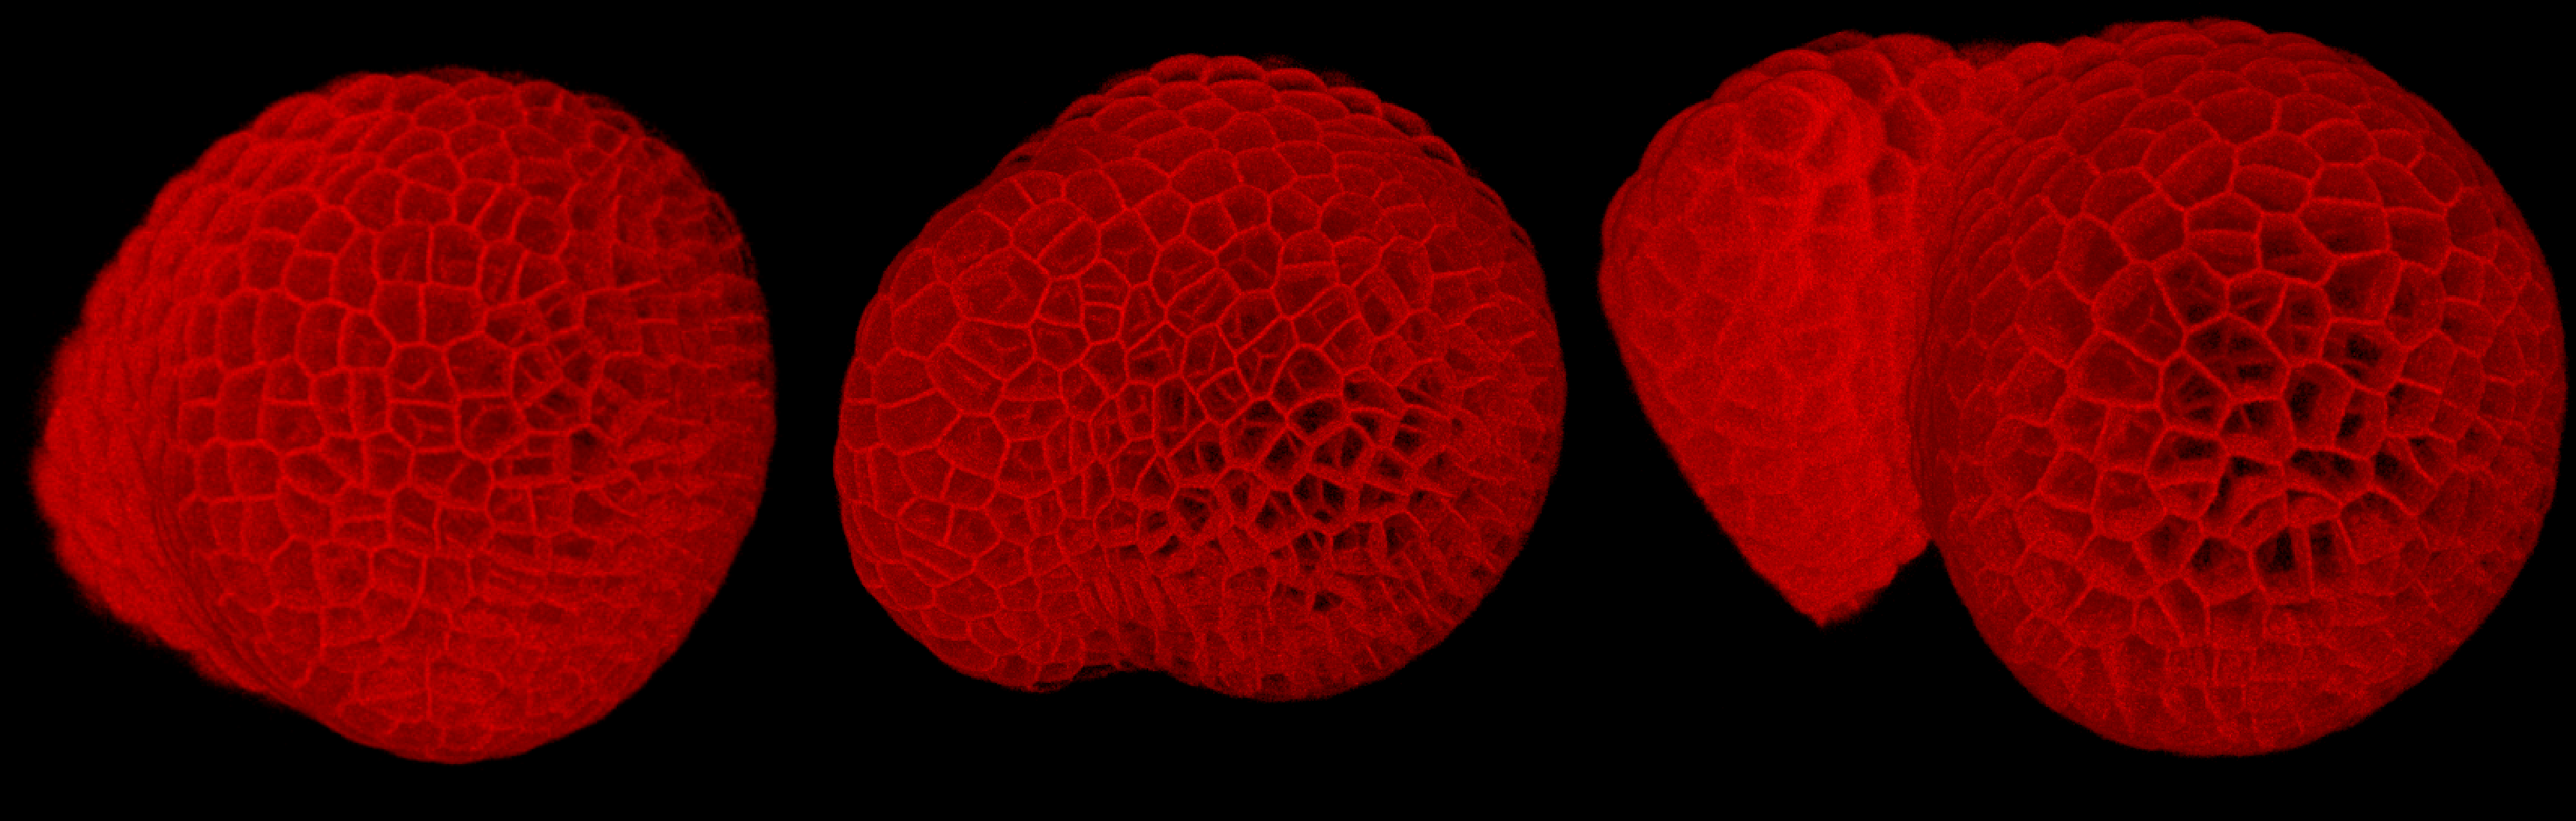
\includegraphics[width=\textwidth]{prim_form.pdf}
  \caption[NPA dilution causes primordia formation]{Membrane channel for plant
    18 at timepoints 0, 36 and 84 hours respectively. In the upper left,
    formation of a primordium throughout the course of the timelapse is clearly
    seen, indicating NPA dilution and reactivation of auxin transport.}
  \label{fig:NPA_primordia}
\end{figure}

\begin{figure}[H]
  \centering
  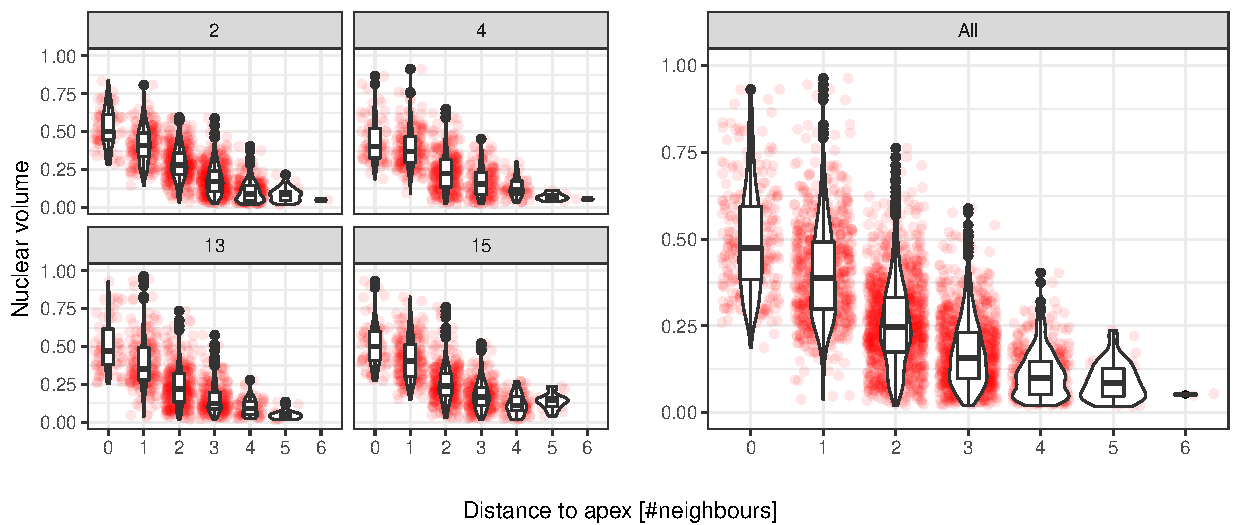
\includegraphics[width=\textwidth]{nvol_apex.pdf}
  \caption[Nuclear volumes at apex]{Distribution of CLV3 nuclear volumes at
    apex, in the epidermis. Lack of data in the periphery is due to CLV3
    loss-of-signal with increasing distance from the CZ. }
  \label{fig:nvol_apex}
\end{figure}

\begin{figure}[H]
  \centering
  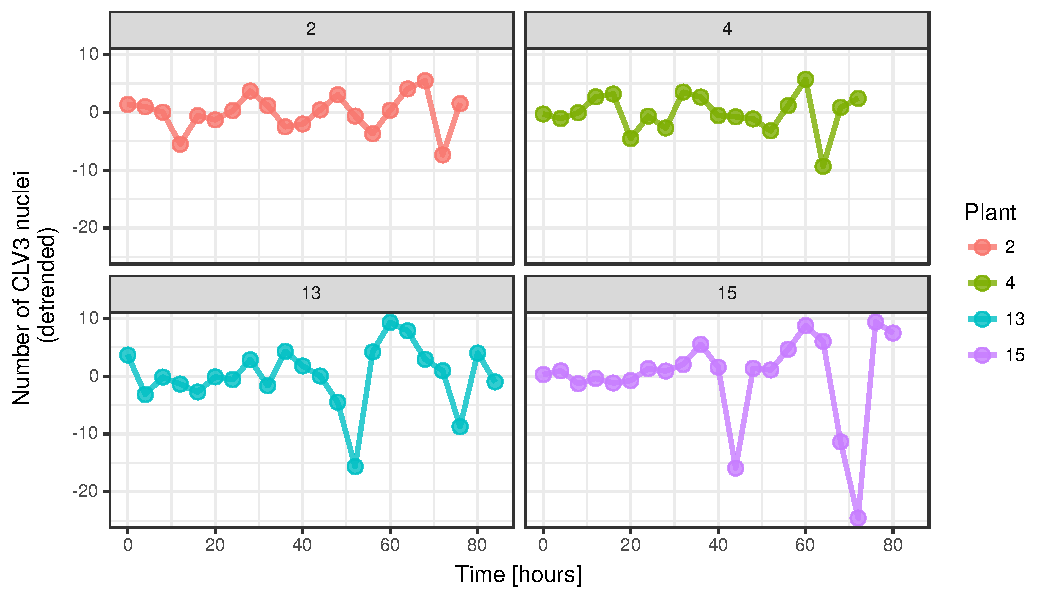
\includegraphics[width=\textwidth]{detrended.pdf}
  \caption[Detrended nuclear trajectories]{Detrended view of trajectories
    visualised in \cref{fig:nNucl_trajectories}}. The detrending is done by
  subtracting the value curve attained by fitting a second order Loess curve to
  each individual nuclear trace.
  \label{fig:detrended}
\end{figure}

\begin{figure}[H]
  \centering
  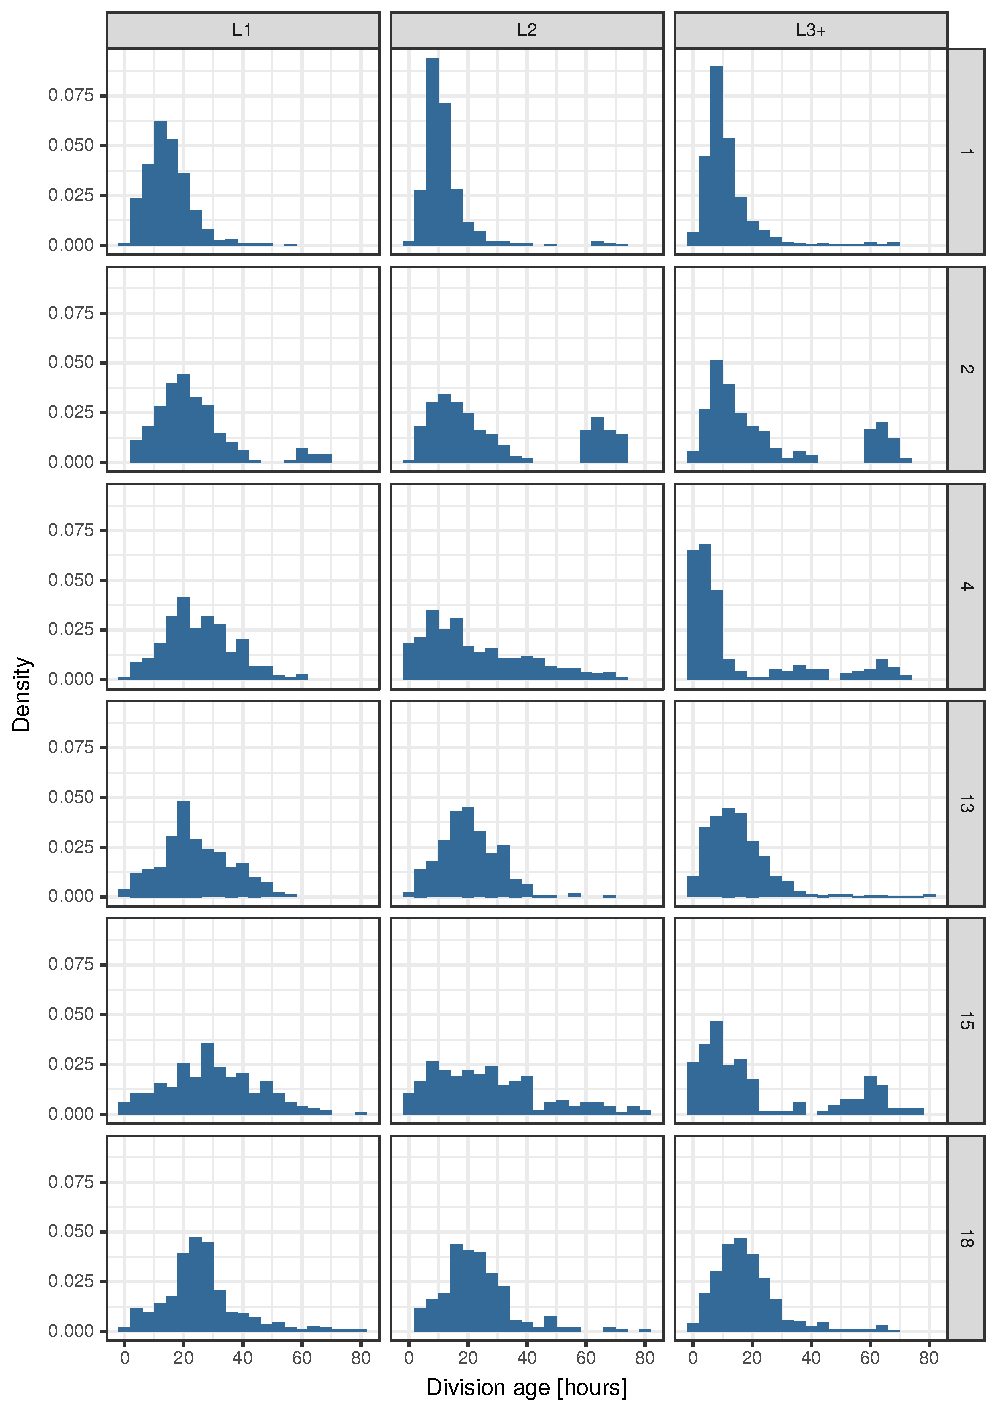
\includegraphics[width=\textwidth]{age_all_plants.pdf}
  \caption[Age distribution, all plants]{Age distribution for all plants,
    showing the general tendency of more cells of higher typically being present
    in the L2 and L3.}
  \label{fig:age_all}
\end{figure}

\begin{figure}[H]
  \centering
  \begin{minipage}[t]{.49\textwidth}
    \centering
    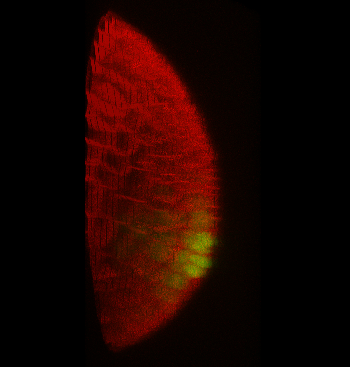
\includegraphics[width=\textwidth]{apexcomp_side.png}
  \end{minipage}
  \begin{minipage}[t]{.49\textwidth}
    \centering
    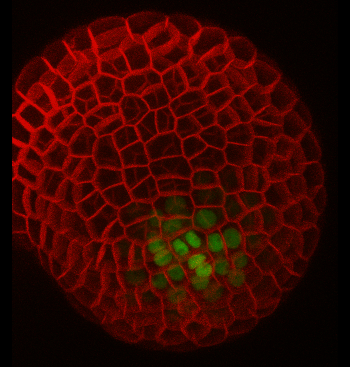
\includegraphics[width=\textwidth]{apexcomp_topview.png}
  \end{minipage}
  \caption[Non-overlapping apices]{Raw data illustration in sideview (left) and
    topview (right). The CLV3 peak expression, defining the CLV3 apex, can be
    seen in green, clearly not coinciding with the geometric apex. Example taken
    plant 4, timepoint 48 hours.}
  \label{fig:apex_center}
\end{figure}

